\chapter{An Introduction to Overture Tool Support for VDM-SL}\label{cha:toolbox}
\initexercise

%\section*{Aims}
\section*{Preamble}

This is an introduction to the Overture Integrated Development Environment (IDE) and its facilities for supporting modelling and analysis in VDM-SL. It may be used as a substitute for Chapter 3 of
``Modelling Systems -- Practical Tools and Techniques in Software Development''\footnote{John Fitzgerald and Peter Gorm Larsen. \emph{Modelling Systems -- Practical Tools and Techniques in Software Development}, Cambridge University Press, 2nd edition 2009.} or as a free-standing guide. Additional material is available on the book's web site~\url{http://overturetool.org/publications/books/ms2/}. Throughout this guide we will refer to the textbook as ``the book'' and the book's web site simply as ``the web site''.

We will use examples based on the \emph{alarm} case study introduced in Chapter~2 of the book. For readers using this as a free-standing guide, an informal explanation of the case study and its
VDM-SL model are given in Appendix~\ref{app:alarm}.

We will introduce the Overture tools during a ``hands-on'' tour of their functionality, providing enough detail to allow you to use Overture for serious applications, including the exercises in the
book. However, this is by no means a complete guide to Overture\footnote{Note that the Overture tool suite support three different VDM dialects; VDM-SL (Specification Language), VDM++ and
  VDM-RT (Real Time) so although this tutorial illustrate how to use Overture with VDM-SL models you will see multiple references to these dialects.}; more information can be obtained from
%
\begin{quote}
\url{www.overturetool.org}.
\end{quote}
%
\section{Introduction}
%
Models in VDM are formal in the sense that they have a precisely described semantics, making it possible to analyse models in order to confirm or refute claims about them. Such an analysis often reveals gaps in the developer's and the client's understanding of the system,
allowing these to be resolved before an expensive commitment is made to program code. The process of analysing claims about systems modelled in this way is termed \emph{validation} and is discussed in greater depth in Chapter~10 of the book.

Section~\ref{sec:install} describes how to obtain the Overture tools.  Section~\ref{sec:vdmsupport} introduces terminology used by Eclipse-based tools like Overture. Section~\ref{sec:templates} describes the features that support the construction and editing of
VDM-SL models.  Section~\ref{sec:debugging} describes the testing and debugging features and Section~\ref{sec:testcov} describes how line coverage information from using the debugger can be extracted and displayed. This is followed in Section~\ref{sec:CT} with an explanation about a combinatorial testing feature available in Overture.  Afterwards Section~\ref{sec:POtool} describes the facilities for automatically generating the checks~(called \emph{proof obligations}) that must be performed in order to ensure that a VDM-SL model is consistent and
meaningful.  Finally, Section~\ref{sec:cmdline} shows how parts of Overture's functionality can be accessed through a command line interface, allowing batch-mode testing. 
%
\section{Getting Hold of the Software}\label{sec:install}
Overture is an open source tool, developed by a community of volunteers and built on the Eclipse platform.  The project to develop the tools is managed using GitHub.  The best way to run Overture is to download a special version of Eclipse with the Overture functionality already pre-installed. If you go to
%
\begin{quote}
\url{http://overturetool.org/}
\end{quote}
%
\noindent you can use the various download links to automatically download pre-built versions of Overture for your operating system.  Supported systems are: Windows, Linux and Mac\footnote{Development of an update facility is planned, which will allow updates to be applied directly from within the generic Eclipse platform without requiring reinstallation. However, this can be a risky process because of the dependencies on non-Overture components and so is not yet supported.}.  Note that when you have extracted all files from the zip file with the Overture executable for your selected operating system you will find the first time you start it up it will ask you to select a workspace. Here we simply recommend you choose the default selected and tick off the box ``Use this as the default and do not ask again''. The first time the application is run, a welcome screen will introduce you to the overall mission of the Overture open source
initiative. 

A large library of sample VDM-SL models, including all those needed for the exercises in the book, is available and can be downloaded from the URL\footnote{The library files are created for use with Eclipse, but can be opened with file compression programs like \texttt{Winrar} on Windows, but it is not necessary to open them at all.}:
%
\begin{quote}
\url{http://overturetool.org/download/examples/Examples-VDMSL.zip}
\end{quote}
%
You can import the example library zip folder as described in Section~\ref{sec:vdmsupport}.  Finally, in order to make use of the test coverage feature described in Section~\ref{sec:testcov} it is necessary to have the text processing system called \LaTeX\ and its \texttt{pdflatex} feature. This can for example be obtained from:
%
\begin{quote}
\url{http://miktex.org/2.9/}
\end{quote}
%
\subsection*{Note for users of \vdmtools$^{\mbox{\small\textbf{{\textregistered}}}}$}
Overture provides a new open source VDM tool set, but it can also work with \vdmtools$^{\mbox{\small\textbf{{\textregistered}}}}$. \vdmtools, originally developed at IFAD A/S, is now maintained and developed by SCSK~(see \url{http://www.vdmtools.jp/en/}). From Overture it is also possible to automatically transfer a project over to \vdmtools.
%
\section{Using the Overture Perspective}\label{sec:vdmsupport}
Eclipse is an open source platform based around a \emph{workbench} that provides a common look and feel to a large collection of extension products. Thus if a user is familiar with one Eclipse product, it will generally be easy to start using a different product on the same workbench. The Eclipse workbench consists of several panels known as \emph{views}, such as the VDM Explorer view at the top left of Figure~\ref{fig:OverturePerspective}. A collection of panels is called a \emph{perspective}, for example
Figure~\ref{fig:OverturePerspective} shows the standard Overture perspective. This consists of views for managing Overture projects and viewing and editing files in an Overture project. The perspectives
available in Overture will be described later, but for the moment think of a perspective as a particular composition of views that is useful for conducting a particular task. Note that the first time
Overture would like to automatically change to a specific perspective it will ask you for permission to do so.  Note also that the first time Overture opens, it is possible that some or all the relevant panels in the perspective are minimized.
%
\begin{figure}[tbh]
\begin{center}
  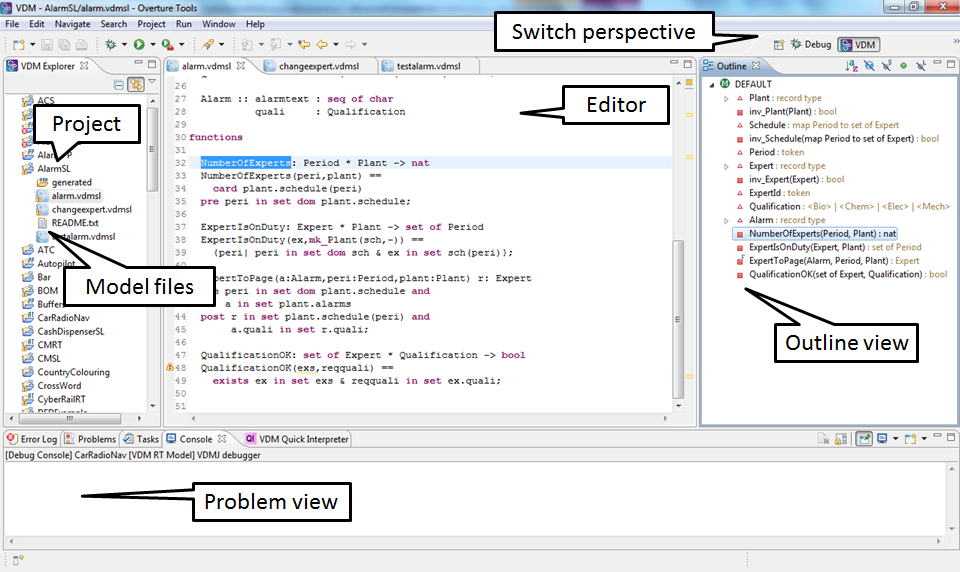
\includegraphics[width=5.5in]{figures/OverturePerspective}
  \caption[labelInTOC]{The Overture Perspective}
  \label{fig:OverturePerspective}
\end{center}
\end{figure}
%
The \emph{VDM Explorer view} allows you to create, select, and delete Overture projects and navigate between the files in these projects. Start by importing the alarm project. This can be done by right-clicking the explorer view and selecting \emph{Import}, followed by \emph{General} $\rightarrow$ \emph{Existing Projects into Workspace}.  In this way the projects from \texttt{examplesSL.zip} file
mentioned above can be imported very easily\footnote{When an existing project is imported in this way, a copy of the original is stored in the current workspace, where all further modifications are reflected.}. Initially it is recommended that you only import the \texttt{AlarmErrSL} and the \texttt{AlarmSL} projects as shown in Figure~\ref{fig:importalarm}\footnote{You need both of these to carry out various exercises throughout this chapter.}.
%
\begin{figure}[!htb]
\begin{center}
  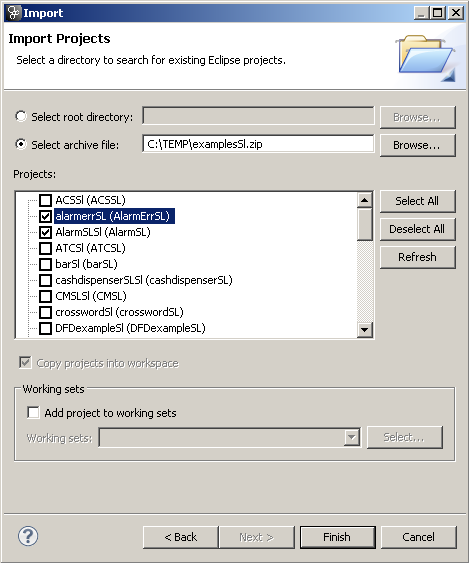
\includegraphics[width=2.5in]{figures/importalarm}
  \caption[labelInTOC]{Importing the \texttt{Alarm} VDM-SL Projects}
  \label{fig:importalarm}
\end{center}
\end{figure}
%
Depending on the dialect of VDM used in a given project, a corresponding Overture editor will be available here. When the \texttt{AlarmSL} project has been imported one can right click on the
project in the \emph{Explorer} view and then select the \texttt{Properties} item in the menu and then
Figure~\ref{fig:settings} will pop up. This includes the properties set for this project and here specific VDM options can be found. Note here that there is a language version option that for the \texttt{AlarmSL} project is set to \texttt{vdm10} which indicates that it includes non-standard features such as {\bf\ttfamily traces}. In addition, options are gathered here for additional checks where the \texttt{AlarmSL} project simply follow the standard settings used for new projects.
%
\begin{figure}[!htb]
\begin{center}
  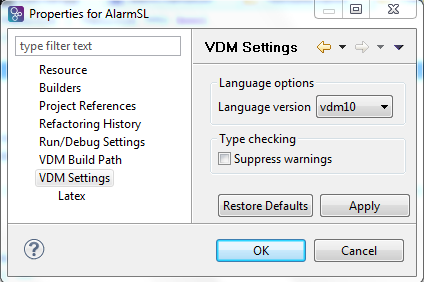
\includegraphics[width=4.0in]{figures/settings}
  \caption[labelInTOC]{Properties for the \texttt{AlarmSL} Project}
  \label{fig:settings}
\end{center}
\end{figure}
%
The \emph{Outline view}, to the right of the editor (see Figure~\ref{fig:OutlineView}), presents an outline of the model in the file selected in the editor. It displays any declared VDM-SL modules, as well as their state components, values, types, functions and operations. In case of a flat VDM-SL model the module is called {\ttfamily{DEFAULT}}.
Figure~\ref{fig:OverturePerspective} shows the outline view on the right hand side. Clicking on an operation or function name will move the cursor in the editor to the definition of the operation or function. At the top of the outline view there is a button to determine what is displayed in the outline view~(it is possible to hide different kinds of definitions, for example).
%
\begin{figure}[!htb]
\begin{center}
  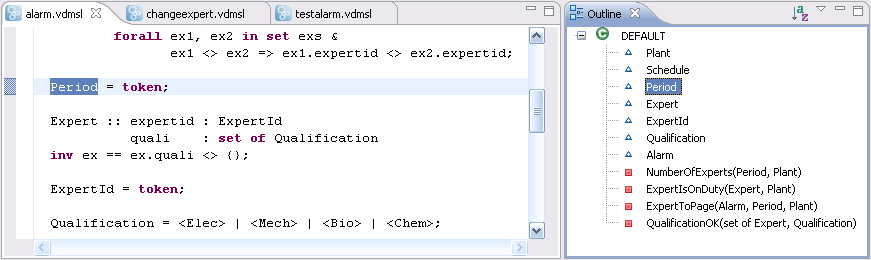
\includegraphics[width=4.5in]{figures/OutlineView}
  \caption[labelInTOC]{The Outline View connected to the Editor view}
  \label{fig:OutlineView}
\end{center}
\end{figure}
%
The \emph{Problems view} displays messages about the projects on which you are working. This includes information generated by Overture, such as warnings and errors. Note that all errors and warnings also appear as tooltips in the VDM-SL editor.

In the standard Overture perspective there is a \emph{VDM Quick Interpreter} view in a pane in the same area as the problems view. This can be used for evaluation of standard VDM expressions independent of all VDM projects incorporated in your Overture IDE. This can be very convenient to gain understanding of the
different VDM operators. In Figure~\ref{fig:QuickIntView} it is possible to see how a couple of expressions (typed in at the box at the bottom of the view) are evaluated\footnote{If errors appear in this evaluation, the current version of the Overture IDE simply yields a \texttt{Fatal error}.  It is anticipated that later releases will provide more helpful run-time error descriptions to the user.}. Note that
in order to get a console where you are able to make use of definitions, you need to use the console launch mode as described in Section~\ref{sec:debugconfig} below. 
%
\begin{figure}[!htb]
\begin{center}
  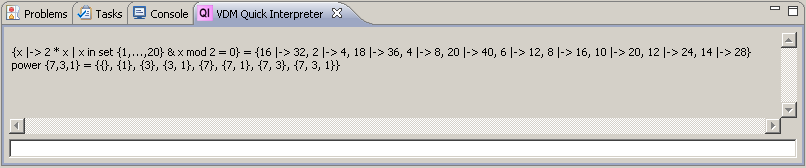
\includegraphics[width=4.5in]{figures/quickinterpreter}
  \caption[labelInTOC]{The VDM quick interpreter view}
  \label{fig:QuickIntView}
\end{center}
\end{figure}
%
Most of the other features of the workbench, such as the menus and toolbars, are similar to those of other Eclipse applications, apart from a special menu with Overture-specific functionality. One convenient feature is a toolbar of shortcuts to switch between different perspectives that appears on the right side of the screen; the shortcuts vary dynamically depending on context and history.
%
\section{Getting Started using Templates}\label{sec:templates}
Before proceeding, please make sure that you have imported both the \texttt{AlarmErrSL} and the \texttt{AlarmSL} projects as shown in Figure~\ref{fig:importalarm}. 
%complete the model of the alarm system. Begin by
%deleting the alarm project in the Overture IDE, and importing the alarm
%project downloaded from the book's web site. This can be done by right
%clicking the project view and selecting \emph{Import}, followed by
%\emph{Existing Projects into Workspace}.
When editing a VDM-SL model, the Overture IDE parses the content of the editor buffer continuously as changes are made. Any parse errors will be reported in the problems view, as well as being highlighted in the editor. See the bottom of Figure \ref{fig:OverturePerspective}. Each time a VDM-SL model file is
saved the editor type-checks the model and reports any errors or warnings. Note also that the suggestions made in the error messages may not always be entirely the action you may wish to take when
correcting the source since the tool cannot guess what you intended to write.

Templates can be particularly useful when modifying VDM-SL models. If you hit the key combination \textit{CTRL+space} after the initial characters of the template needed, Overture triggers a proposal. For example, if you type ''fun'' followed by \textit{CTRL+space}, the Overture IDE will propose the use of an implicit or explicit function template as shown in Figure~\ref{fig:functionTemplate}. The Overture IDE supports several types of template: cases, quantifications, functions (explicit/implicit), operations (explicit/implicit) and many more\footnote{It is possible to see and enhance the complete list of these by selecting \emph{Window} $\rightarrow$ \emph{Preferences} $\rightarrow$ \emph{VDM}  $\rightarrow$ \emph{Templates}.}. Additional templates can easily be added in the future. The use of templates makes it much easier for users lacking deep familiarity with VDM's syntax to nevertheless construct models.
%
\begin{figure}[!htb]
\begin{center}
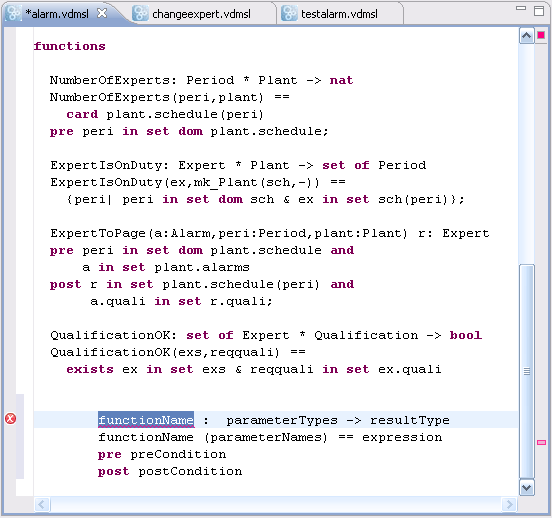
\includegraphics[width=4in]{figures/FunctionTemplate}
\caption{Explicit function template}
\label{fig:functionTemplate}
\end{center}
\end{figure}

A new VDM-SL project is created by choosing \emph{File} $ \rightarrow$ \emph{New} $\rightarrow$ \emph{Project}. The dialog box shown in Figure~\ref{fig:newOvertureProjectSL} will appear. Ensure that VDM-SL is selected as the project type, click \emph{Next} and then name the project \texttt{Test}.  If \emph{Next} is clicked again, it becomes possible to link the new project to projects already in the workspace.  Clicking \emph{Next} again allows you to select standard libraries as shown in Figure~\ref{fig:stdlibs}. These standard libraries require users to make use of modules but in return it is possible to get standard input/output, math and general utility functionality by selecting the appropriate standard libraries. In this \texttt{Test} project we can try to select the \texttt{IO} standard library. Afterwards one simply clicks \texttt{Finish}. Now you have an almost empty project (with the exception of the \texttt{IO.vdmsl} file in the \texttt{lib} directory) and you can then
either add new VDM-SL files to the project or simply paste in existing VDM-SL source files from elsewhere. Adding a VDM-SL file to a project you can right click on the project and then select \emph{New} $\rightarrow$ \emph{VDM-SL Module} and then give a meaningful name (e.g.\ \texttt{Test}) to
the module you would like to start defining and press \texttt{Finish}. This will create a new file with a module with the selected name and with space for the different kinds of definitions you can make inside such a VDM-SL module.
%
\begin{figure}[!htb]
\begin{center}
  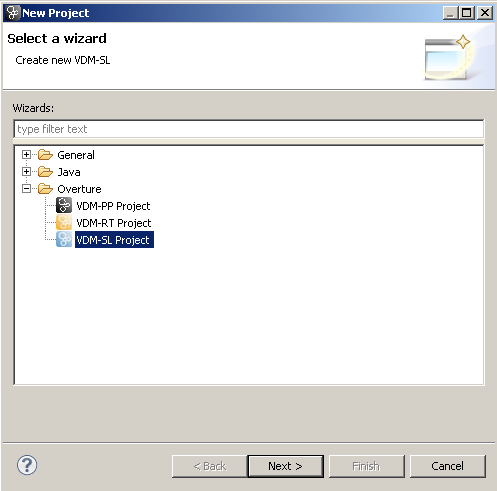
\includegraphics[width=2.5in]{figures/newovertureSLproject}
  \caption[labelInTOC]{Creating a New VDM-SL Project}
  \label{fig:newOvertureProjectSL}
\end{center}
\end{figure}

\begin{figure}[!htb]
\begin{center}
  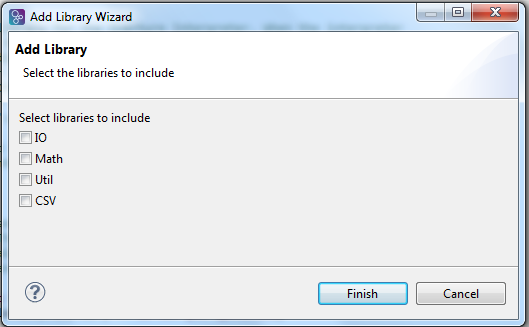
\includegraphics[width=2.5in]{figures/stdlibs}
  \caption[labelInTOC]{The VDM-SL Standard Libraries}
  \label{fig:stdlibs}
\end{center}
\end{figure}
%
\begin{myexercise}\label{ex:tb-error}
Try to create a new \texttt{Test} VDM-SL project and update the \texttt{test.vdmsl} file before {\bf\ttfamily{exports all}} with:
%
\begin{vdmsl}
imports from IO all
\end{vdmsl}
%
in order to make use of the IO standard library in the \texttt{Test} module. Inside \texttt{IO} there is for example a definition of a function called \texttt{print} and that can for example be used in an
operation as: 
%\newpage
\begin{vdmsl}
Try: nat ==> nat
Try(n) ==
  (IO`print(n);
   return n + 1)
\end{vdmsl}
%
Insert this and later on when you have learned how to create a debug configuration you can try to see what happens when \texttt{Try} is debugged. 
\end{myexercise}
%
\section{Debugging}\label{sec:debugging}
This section describes facilities for debugging a model by stepping through the evaluation of functions and operations. The alarm example is used. The following test file (\texttt{testalarm.vdmsl}) can be found in the alarm project and it is provided in Appendix~\ref{sec:VDMModel}. 
%
%\lstset{language=VDM-SL}
%\input{testalarm.vdmsl}

By using the values defined in this test file, it is possible to exercise the system in order to check whether, for this test, the correct expert is paged as a result of a given alarm.
%
\subsection{The Debug configuration}\label{sec:debugconfig}
Before debugging can be initiated in Overture
%%\footnote{In the
%  current version of Overture we advise to use the \texttt{clean}
%  feature that can be activated by right clicking the project and
%  selecting \texttt{Clean}. This will make sure that proper type
%  checking is conduction prior to debugging.}
, a debug configuration must be created by right-clicking the project and choosing \emph{Debug As} $ \rightarrow $ \emph{Debug configuration}.  In the resulting window, locate and click on the \texttt{AlarmSL} project in the left pane.
%\footnote{Note that the
%  \emph{Run As} functionality existing Eclipse users are used to is
%  not supported in the current version of Overture.}. 

The debug configuration dialog has 3 different launch modes:
%
\begin{description}
\item[Entry Point:] This is the standard Eclipse approach where one decides before debugging which operation/function to call.
\item[Remote Console:] This is an advanced option that enables remote control of the interpreter and is described in the Overture user manual~\cite{Larsen&13a}.
\item[Console:] This will simply start up a console where the user can interactively debug different operations/functions defined in the selected project\footnote{For VDMTools users this will be a familiar console corresponding to a VDM model that has been initialised in VDMTools' interpreter.}.
\end{description}
%
Here we will start by using the traditional Eclipse approach with an ``Entry Point'' launch configuration which requires the project name, the class and the operation/function used as the entry point of the test. When the \texttt{AlarmSL} project was imported you also automatically got a basic launch configuration called \texttt{AlarmSL}. This one simply calls \texttt{Run(e1)} but you can change it to call something else by chosing a different function from the Browse dialog.
Figure~\ref{fig:debugConfiguration} shows the \texttt{AlarmSL} debug configuration for the alarm model. Note the three different debug options here. Two of these are not explained further here but the one called \texttt{Generate Coverage} is important for you to check in case you would like to collect test coverage information as explained below in Section~\ref{sec:testcov}. The class and operation/function
name can be chosen from a Browse dialog; if the operation or function has arguments, these must be typed in manually between the brackets of the entry point function/operation. If this is not well-typed, such that the overall expression is type correct, an error will be shown at the top of the debug configuration window. This means that one needs to change the \emph{Operation} line for example from:
%
\begin{vdmsl}
NumberOfExperts((Period) peri, (Plant) plant)
\end{vdmsl}
%
\noindent to for example:
%
\begin{vdmsl}
NumberOfExperts(p2, plant1)
\end{vdmsl}
%
\begin{figure}[htp]
\begin{center}
  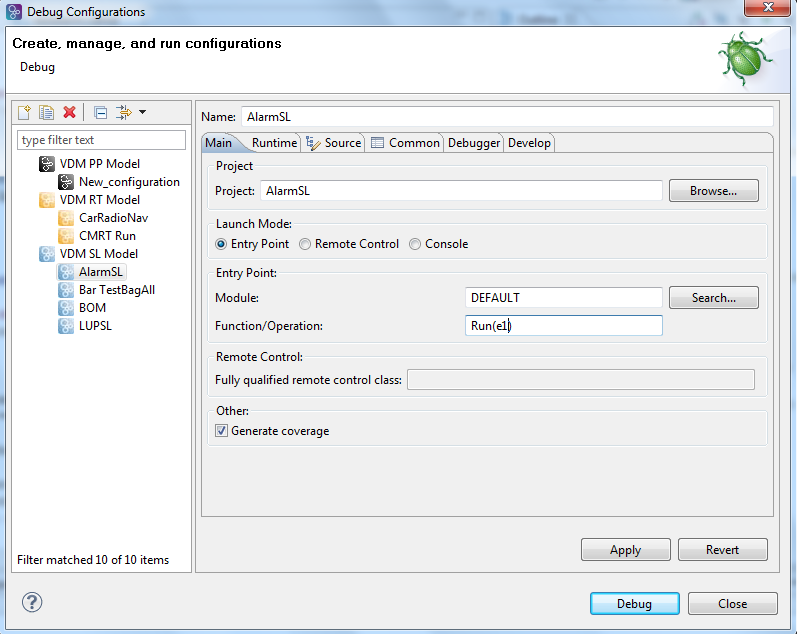
\includegraphics[width=4in]{figures/debuglauncer}
  \caption{The debug configuration dialog}
  \label{fig:debugConfiguration}
\end{center}
\end{figure}
%
Once the configuration is ready, the model can be debugged. If one has already set a breakpoint on one of the lines that will be executed, this will change the main perspective of the Overture IDE to the \emph{Debug perspective}. If no breakpoints are set the result is simply shown in the \emph{Debug Console} view in the lower part of the Overture perspective. Breakpoints can easily be set by double clicking in the left margin in the editor view. When the debugger reaches the location of a breakpoint, evaluation suspends and the user can inspect the values of variables and step through the VDM-SL model line by line. So for \texttt{NumberOfExperts} (in the main model file) try to set such a breakpoint on line 34\footnote{Line numbers can be added in the editor by right clicking in the left-hand-side margin of the editor view and selecting \texttt{Show Line Numbers}.}
and debug again.
%
\subsection{The Debug Perspective}
%The \emph{Debug perspective} shows the VDM model in an editor, like the
%Overture perspective, along with other specialized views for debugging.
The Debug perspective is illustrated in Figure~\ref{fig:DebuggingVDM}.
%
\begin{figure}[htp]
\begin{center}
  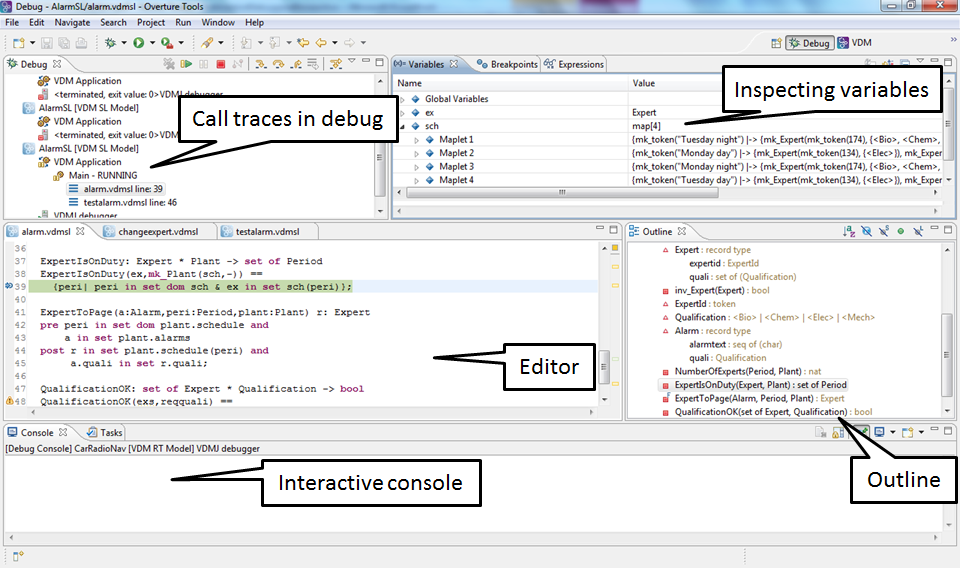
\includegraphics[width=4.5in]{figures/DebuggingVDM}
  \caption[Debugging perspective]{Debugging perspective}
  \label{fig:DebuggingVDM}
\end{center}
\end{figure}
%
The \emph{Debug view} is located in the upper left corner of the Debug perspective. It shows all running models and the call stacks belonging to them. It also shows whether a given model is stopped, suspended or running. 
% All threads are also shown, along with their running
% status. It is possible to switch between threads from the Debug view.
%
\begin{table}
\begin{center}
\begin{tabular}{|l|l|}\hline \hline
\textbf{Button} & \textbf{Explanation} \\ \hline

\includegraphics[width=0.03\textwidth]{figures/resume} & Resume debugging \\

\includegraphics[width=0.03\textwidth]{figures/suspend} & Suspend debugging\\

\includegraphics[width=0.03\textwidth]{figures/terminate} & Terminate debugging\\

\includegraphics[width=0.03\textwidth]{figures/stepinto} & Step into\\

\includegraphics[width=0.03\textwidth]{figures/stepover} & Step over \\

\includegraphics[width=0.03\textwidth]{figures/stepreturn} & Step return\\

\includegraphics[width=0.03\textwidth]{figures/stepbystep} & Use step filters\\
\hline \hline
\end{tabular}
\caption{Overture debugging buttons\label{tab:debugButtons}}
\end{center}
\end{table}
%
At the top of the view are buttons for controlling debugging such as; stop, step into, step over and resume. These are standard Eclipse debugging buttons (see Table~\ref{tab:debugButtons}).

The \emph{Variables view} shows all the variables in a given context when a breakpoint is reached. The variables and their displayed values are automatically updated when stepping through a model. The view is
located in the upper right hand corner in the Debug perspective.
%It is also possible to inspect complex
%variables, expanding nested arrays and so on.
%
\begin{figure}[htp]
\begin{center}
  \caption{Breakpoint View}
  \label{fig:BreakpointView}
  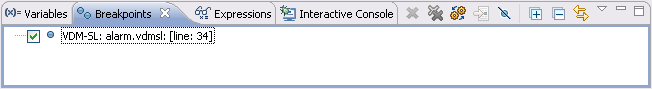
\includegraphics[width=4in]{figures/BreakpointView}
\end{center}
\end{figure}
%
\subsection{Breakpoints}
The \emph{Breakpoints view} gives an overview of all breakpoints set~(see Figure~\ref{fig:BreakpointView}). From this view you can navigate to the location of a given breakpoint, disable or delete it, or set its properties.
%In figure
%\ref{fig:DebuggingVDM} the Breakpoints view is hidden behind the
%Variables view in the upper right hand corner in a tabbed notebook. 
Conditional breakpoints are supported. These are a powerful tool for the developer since they allow you to specify a condition that must be true in order for the debugger to stop at the given breakpoint. The
condition can either be a boolean expression using variables in scope at the breakpoint, or it can be a hit count after which the breakpoint should become active.
%
\begin{figure}[htp]
\begin{center}
  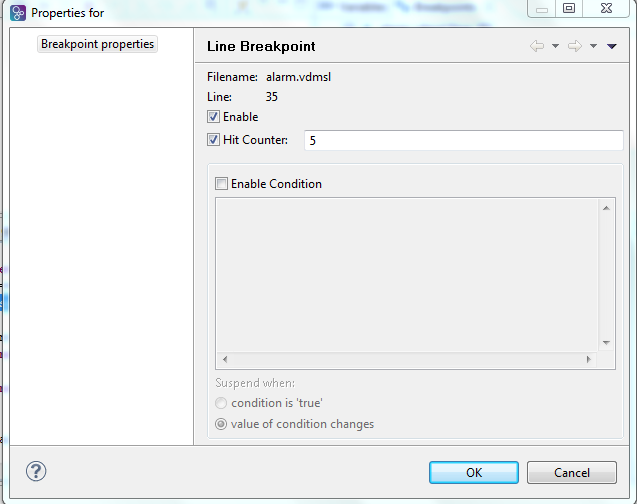
\includegraphics[width=4in]{figures/Breakpointconditional}
  \caption{Conditional breakpoint options}
  \label{fig:BreakpointConditional}
\end{center}
\end{figure}
%
You can make a simple breakpoint conditional by right clicking on the breakpoint mark in the left margin of the editor and selecting the option \emph{Breakpoint properties}. This opens a dialog shown in
Figure~\ref{fig:BreakpointConditional}.
%It is possible to choose
%between two different types of conditional: a hit count condition and one based
%on an expression defined by the user.

The \emph{Expressions view} allows you to enter \emph{watch} expressions whose values are automatically displayed and updated when stepping. ``Watch expressions'' can be added manually or created by selecting \emph{create watch expression} from the Variables view. It is possible to edit existing expressions.  Like the Breakpoints view, this view is hidden in the upper right hand corner in Figure~\ref{fig:DebuggingVDM}.  Views which are not currently displayed can be opened from the menu \emph{Window} $\rightarrow$ \emph{Show View}.  When you are finished debugging, you can switch back to the VDM perspective (this does not happen automatically when debugging stops).
%While the Expressions view allows you to inspect values, its
%functionality is somewhat limited. For more thorough inspections, the
%\emph{Interactive Console view} is provided. Here commands can be
%executed in a given context, i.e.\ when the debugger is at a
%breakpoint. The Interactive Console keeps a command history so that
%previously executed commands can easily be run again. The interactive
%console can be seen at the bottom of
%Figure~\ref{fig:DebuggingVDM}.

\begin{myexercise}
\label{ex:tool-monitor}Use the interpreter to evaluate the
  following expressions:
\begin{vdmsl}
NumberOfExperts(p2,plant1)
NumberOfExperts(p3,plant1)
ExpertIsOnDuty(e1,plant1)
ExpertIsOnDuty(e2,plant1)
ExpertIsOnDuty(e3,plant1)
\end{vdmsl}
%Rising([34,67,45,120,7])
%OverLimit([333,321,345,399,357])
%OverLimit([457,421,387,366,340])
%OverLimit2([457,421,387,366,340])
\end{myexercise}
%
\section{Test coverage}\label{sec:testcov}
It is often useful to know how much of a model has been exercised by a set of tests\footnote{Note that this feature is not yet supported for models using unicode characters such as Japanese identifiers.}. 
This gives some insight into the thoroughness of a test suite and may also help to identify parts of the model that have not been assessed, allowing new tests to be devised to cover these. When any evaluation is performed on a VDM-SL model, the interpreter records the lines of the VDM-SL model that are executed. This permits the line coverage to be examined after a test to identify the parts of the
VDM-SL model that have not yet been exercised -- coverage is cumulative, so a set of tests can be executed and their total coverage examined at the end.

In our simple example, the different tests in the exercise above do cause the majority of the VDM-SL model to be executed, but for demonstration purposes let us start by cleaning the model (select the project in the VDM Explorer panel and select \texttt{Clean} from the \texttt{Project} menu). If we simply take the \texttt{AlarmSL} debug launch configuration, the \verb|ExpertIsOnDuty| function in \verb|alarm.vdmsl| is called by the \texttt{Run} function. Remember that whenever test coverage information is desired, the \texttt{Generate Coverage} option must be selected as shown in Figure~\ref{fig:debugConfiguration}.  Once the debugger has completed and the result is written out in the \texttt{console}, it is possible to right click on the \texttt{AlarmSL} project and select the \emph{Latex} $\rightarrow $ \emph{PdfLatex} option.  The coverage information that has been gathered about any expressions that have been debugged since the last change to a file was saved, or the project was cleaned, will be turned into a pdf file. The \texttt{AlarmSL.pdf} file is placed in the \texttt{generated/latex} directory as shown in Figure~\ref{fig:testcov}, and it includes the VDM definitions from all the files included in the project, including coverage information. Note that whenever the model is adjusted, or it is cleaned so that it is type checked again, all the files in the \texttt{generated} directory are deleted.
%
\begin{figure}[tb]
\begin{center}
\resizebox{.4\textwidth}{!}{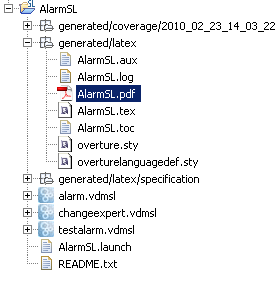
\includegraphics{figures/generatedpdf}}
\end{center}
\caption{The generated pdf file with test coverage information\label{fig:testcov}}
\end{figure}
%
The coverage information is provided in such a way that expressions not covered are shown in red in the generated pdf file. In addition, after the contents of each VDM-SL source file, a table with coverage overview is provided for that file. For the \texttt{alarm.vdmsl} file this looks like:
%
\begin{longtable}{|l|r|r|}
\hline
Function or operation & Coverage & Calls \\
\hline
\hline
ExpertIsOnDuty & 100.0\% & 1 \\
\hline
ExpertToPage & 0.0\% & 0 \\
\hline
NumberOfExperts & 0.0\% & 0 \\
\hline
QualificationOK & 100.0\% & 12 \\
\hline
\hline
alarm.vdmsl & 64.0\% & 13 \\
\hline
\end{longtable}
%
\noindent where the \texttt{ExpertIsOnDuty} function is fully covered by just one call (due to the fact that its body is simply one line) and here the \texttt{QualificationOK} function is called 12 times
because it is used inside the invariant of the \texttt{Plant} type\footnote{Note that the coverage from the combinatorial testing feature described in Section~\ref{sec:CT} is not taken into account in the current version of the Overture IDE, but this will be enabled in a later release.}.
%
%It is often useful to know how much of a model has been exercised by a
%set of tests. This gives some insight into the thoroughness of a test
%suite and may also help to identify parts of the model that have not
%been assessed, allowing new tests to be devised to cover
%these. VDMTools has a facility to support this kind \emph{code
%  coverage}, similar to the tools that already exist for many
%programming languages. In Overture, special commands can be used
%in the \textsf{\small Dialog} part of the interpreter
%sub-window. There is a command called \texttt{tcov} that can be used
%with arguments to reset the coverage information, to read and write
%the coverage information to a file. The \texttt{rtinfo} command takes
%such a coverage file for the VDM model in question and presents
%information about the percentage of coverage for each function, as
%well as data on the number of times each function is
%called. Figure~\ref{fig:testcov} illustrates how this can be done with
%the alarm example. Even more detailed information at subexpression
%level can be shown if the VDM model is pretty-printed but this
%requires special commands depending upon the format used for the VDM
%model. In order to see how this is done, refer to the user manual for
%VDMTools \cite{UserMan}.
%
\section{Combinatorial Testing}\label{sec:CT}
The previous sections have shown how to test and debug models manually. However, Overture also contains a feature enabling more automation in the testing process, making more comprehensive high-volume testing feasible. It is possible to write regular expressions, known as \emph{traces}, which expand into a large set of individual tests.

In order to illustrate how this can be used, we extend the \texttt{testalarm.vdmsl} file with a few definitions illustrating the principles. However, the value of this feature is most significant
when we deal with operations that update state components, because then test sequencing is important in detecting more subtle errors. When new traces are incorporated in a VDM project, you may need
to press the \textsf{Refresh} button (
\includegraphics[width=0.02\textwidth]{figures/refresh}) in the
\emph{CT Overview} view.

In order to do the automation, Overture needs to know about the combinations of function calls that you would like to have carried out, so it is necessary to write a kind of regular expression called a
\emph{trace} in the VDM-10 version. VDM-SL has been extended such that traces can be written directly as a part of a VDM-SL model. Here the definition looks like:
%
\begin{vdmsl}
traces

  Test1: let a in set alarms
         in
           let p in set ps 
           in
             (NumberOfExperts(p,plant1);
              pre_ExpertToPage(a,p,plant1);
              let ex in set exs
              in
                post_ExpertToPage(a,p,plant1,ex))
               
  Test2: let ex in set exs
         in
           ExpertIsOnDuty(ex,plant1)
\end{vdmsl}
%
\begin{figure}[htbp]
\begin{center}
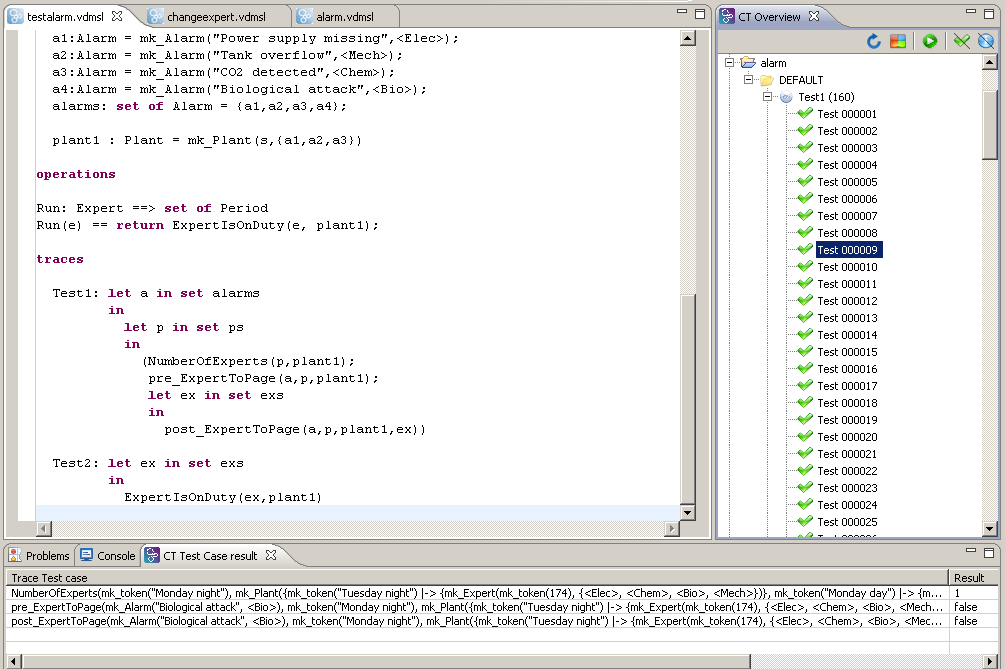
\includegraphics[width=5.5in]{figures/tracesalarm}
\caption{Using Combinatorial Testing for the Alarm VDM-SL model\label{fig:stracesalarm}}
\end{center}
\end{figure}
%
\noindent The nested let-be statements in the trace called \texttt{Test1} yield all possible combinations of their variable bindings whereas manual debugging will just select a few combinations. The cardinality of these sets determines the overall number of test cases, each being formed as a sequence of three function calls, where the last one is nested inside a new let-be expression. In this case, the cardinality of the three sets are respectively 4 (\texttt{alarms}), 5 (\texttt{ps}) and 8 (\texttt{exs}). Multiplying these gives 160. If you select the Combinatorial Testing perspective you will see the \textsf{CT Overview} view. Inside this view you can select the alarm project, right click it and choose the \textsf{Full Evaluation} option as shown in Figure~\ref{fig:CToptions}.  Now Overture expands and executes all 160 test cases one after another. The results of these executions are illustrated with green
check marks and red crosses, meaning that the tests passed or failed respectively.  See Figure~\ref{fig:stracesalarm}. In this case we only get green check marks but you can try to extend the traces making use of the \texttt{ChangeExpert} function from Exercise~\ref{ex:tool-alarm} and possibly find errors in that. Note that in the Combinatorial Testing perspective, the view in the lower region is able to show the individual steps of a selected test case, along with the corresponding results from its three function calls.
%
\begin{figure}[htbp]
\begin{center}
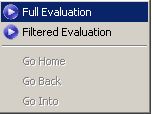
\includegraphics[width=1.5in]{figures/CToptions}
\caption{Invoking the combinatorial testing feature\label{fig:CToptions}}
\end{center}
\end{figure}
%
The syntax for traces also enables function/operation repetition and alternatives to be specified, but these were not needed for this simple case. Using the full power of traces, it is possible to efficiently generate and execute very large test suites. Naturally, this is most likely to find inconsistencies when the model violates its essential predicates (invariants, pre and post-conditions)\footnote{Note that when using repetitions and sequencing in combination it is easy to define traces that expand to hundreds of thousands of test cases, and naturally their execution may then be very slow if one executes them all.}.

\section{Proof Obligations}\label{sec:POtool}

Overture can also generate \emph{Proof Obligations} for a VDM-SL model. These are boolean expressions which highlight areas of the VDM-SL model where some constraint must be met in order to guarantee internal consistency (i.e.\ no run-time errors will occur while debugging if these are all satisfied). This includes type and class invariants or function or operation pre/post conditions. Each proof
obligation should evaluate to \emph{true}. Proof obligations are explained in detail in Chapter~10.

This feature is invoked by right clicking on the project in the \emph{Explorer view} and then selecting the \emph{Proof Obligations} \texttt{->} \emph{Generate Proof Obligations} entry. This will start up a proof obligation perspective with a special \emph{PO view}. For the alarm example this view looks like that in Figure~\ref{fig:POview}.
%
\begin{figure}[htbp]
\begin{center}
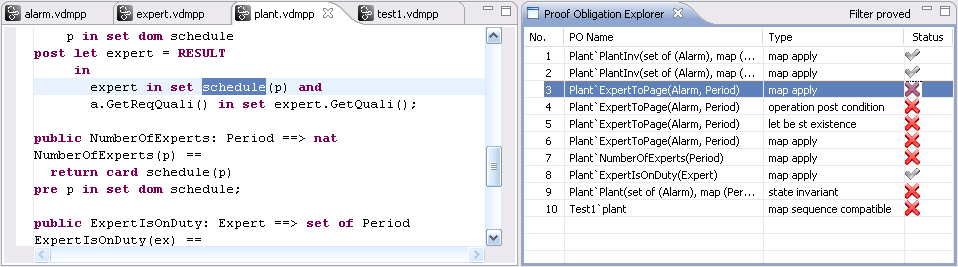
\includegraphics[width=5.5in]{figures/poview}
\caption{The Proof Obligation view for the Alarm VDM-SL model\label{fig:POview}}
\end{center}
\end{figure}
%
Here the eighth proof obligation is related to the satisfiability of the \texttt{ExpertToPage} function which is defined as follows: 

\begin{vdmsl}
ExpertToPage(a:Alarm,peri:Period,plant:Plant) r: Expert
  pre peri in set dom plant.schedule and
      a in set plant.alarms
  post r in set plant.schedule(peri) and
       a.quali in set r.quali;
\end{vdmsl}

%Proof obligations can be produced either automatically from the command line
%with the \verb|-p| option, or they can be generated from the interactive prompt
%using the \verb|pog <function/operation>| command. In the case of our alarm
%example, most of the proof obligations concern the invariant on the Plant when
%changes of state occur, or the application of various map types, where the key
%being mapped must exist in the domain of the map. The \texttt{Test1} class itself also
%produces an obligation, meaning that we must verify that the two maplets in the
%Plant test data supplied are compatible:

Here the proof obligation records the constraint that, for all possible arguments satisfying the pre-condition, the post-condition allows at least one possible valid result of the function. This is described as a proof obligation as follows: 

\begin{vdmsl}
(forall a:Alarm, peri:Period, plant:Plant &
    pre_ExpertToPage(a, peri, plant) => 
    exists r:Expert & post_ExpertToPage(a, peri, plant, r))
\end{vdmsl}

In general, users check proof obligations by inspecting the VDM-SL model, though new Overture tools are being developed to check the majority of proof obligations automatically using formal proof and related
techniques. You can also note in Figure~\ref{fig:POview} that in the \emph{Proof Obligation Explorer} view there is a status field and in there a few of the proof obligations have a checkmark. This is used to indidate that these proof obligations are trivially satisfied. It is also possible to get rid of such proof obligations in the list by pressing the \emph{Filter proved} button at the top of the \emph{Proof Obligation Explorer} view.
%
\section{A Command-Line Interface}\label{sec:cmdline}
So far only the graphical user interface of Overture has been presented, but the core of Overture also
provides a simple command line interface.  This is useful for the automatic batch execution of tests, though the command line also provides a full set of interactive execution and debugging commands which can be useful when examining batch tests. 

Overture is written in Java, and so to run it from the command line, the Overture jar file\footnote{See the Overture documentation at \url{http://overturetool.org/documentation/manuals.html} for the location of the \texttt{jar} file or use the script or Windows \texttt{bat} file incorporating this.} should be executed with a Java JRE (version 7 or later):

\lstset{style=tool,language=}
\begin{lstlisting}
java -jar Overture-2.3.0.jar
\end{lstlisting}

\noindent If the jar file is executed with no further options like this, it will print a list of available options and exit. The most important option is the VDM dialect that the tool should use. In the
case of our alarm example, we want to use VDM-SL for which the option is \verb|-vdmsl|. After this, we can simply specify the names of the VDM-SL model files to load, or the name of a directory from which to
load all VDM-SL model files:

\begin{lstlisting}
java -jar Overture-2.3.0.jar -vdmsl AlarmSL
\end{lstlisting}

\noindent In this case, this is the location of the imported AlarmSL project in the workspace directory selected when Overture first started up.  This will perform a syntax and type check of all the VDM-SL model files in the \texttt{AlarmSL} directory, producing any errors and warning messages on the console, before terminating:

\begin{lstlisting}[style=mystyle]
Parsed 1 module in 0.11 secs. No syntax errors
Type checked 1 module in 0.093 secs. No type errors
\end{lstlisting}

\noindent In the case of our alarm example, there are no syntax or type errors. Any warnings can be suppressed using the \verb|-w| option.

If a VDM-SL model has no type errors, it can either be given an expression to evaluate as an option on the command line, or the user can enter an interactive mode to evaluate expressions and debug their execution.

To evaluate an expression from the command line, the \verb|-e| option is used, followed by a VDM expression to evaluate. You may also find the \verb|-q| option useful, as this suppresses the informational messages about the parsing and type checking:

\begin{lstlisting}[style=tool]
java -jar Overture-2.3.0.jar -vdmsl -q -e 
     "ExpertIsOnDuty(e1, plant1)" AlarmSL
\end{lstlisting}

\noindent This produces a single line of output for the evaluation, since the parsing and checking messages are suppressed, and there are no warnings:

\begin{vdmsl}
{mk_token("Monday day"), mk_token("Tuesday day")}
\end{vdmsl}

Clearly a batch of test evaluations could be performed automatically by running a series of similar commands and saving the output results for comparison against expected results.

To run the command line interpreter interactively, the \verb|-i| command line option must be given. Instead of terminating after the type check, this will cause Overture to enter its interactive mode, and
give the interactive \verb|>| prompt:

\begin{lstlisting}[style=tool]
Parsed 1 module in 0.14 secs. No syntax errors
Type checked 1 module in 0.11 secs. No type errors
Initialized 1 module in 0.094 secs. 
Interpreter started
>
\end{lstlisting}

\noindent From this prompt, various interactive commands can be given to evaluate expressions, debug their evaluation, or examine the VDM-SL model environment.  The \verb|help| command lists the commands
available. The \verb|quit| command leaves the interpreter. For example, the following session illustrates the evaluation of a \verb|Run| operation, and a debug session with a breakpoint at the start of the same operation:

\begin{minipage}{ \linewidth}
\begin{lstlisting}[style=tool]
> print Run(e1)
= {mk_token("Monday day"), mk_token("Tuesday day")}
Executed in 0.015 secs.

> break ExpertIsOnDuty
Created break [1] in 'DEFAULT' (AlarmSL\alarm.vdmsl) 
at line 39:6
39:{peri| peri in set dom sch & ex in set sch(peri)};
> print Run(e1)
Stopped break [1] in 'DEFAULT' (AlarmSL\alarm.vdmsl) 
at line 39:6
39:{peri| peri in set dom sch & ex in set sch(peri)};
[MainThread-9]> print sch
sch = {mk_token("Tuesday night") |->
 {mk_Expert(mk_token(174), {<Elec>, <Chem>, 
                            <Bio>, <Mech>})},
  mk_token("Monday day") |->
 {mk_Expert(mk_token(181), {<Elec>, <Mech>}),
  mk_Expert(mk_token(169), {<Chem>, <Bio>}),
  mk_Expert(mk_token(134), {<Elec>})},
 mk_token("Monday night") |->
 {mk_Expert(mk_token(174), {<Elec>, <Chem>, 
                            <Bio>, <Mech>})},
  mk_token("Tuesday day") |->
 {mk_Expert(mk_token(134), {<Elec>}),
  mk_Expert(mk_token(154), {<Bio>, <Chem>, <Elec>}),
  mk_Expert(mk_token(190), {<Mech>, <Bio>})}}
[MainThread-9]> continue
= {mk_token("Monday day"), mk_token("Tuesday day")}
Executed in 18.281 secs. 
> 
\end{lstlisting}
\end{minipage}

\noindent Notice that the \verb|print| command is available at the breakpoint to examine the runtime state of the system. In the example, we print out the value of the \verb|sch| variable. The \verb|help|
command is context sensitive, and will list the extra debugging commands available at a breakpoint, such as \verb|continue|, \verb|step|, \verb|stack|, \verb|list| and so on. The full set of commands is described in the Overture User Guide\footnote{Supplied with the Overture documentation.}.

%\begin{lstlisting}
%> coverage AlarmSL/alarm.vdmsl
%...
%NumberOfExperts: Period * Plant -> nat
%NumberOfExperts(peri,plant) ==
%-  card plant.schedule(peri)
%-pre peri in set dom plant.schedule;
%
%ExpertIsOnDuty: Expert * Plant -> set of Period
%ExpertIsOnDuty(ex,mk_Plant(sch,-)) ==
%+  {peri| peri in set dom sch & ex in set sch(peri)};
%...
%> latex AlarmSL/alarm.vdmsl
%Latex coverage written to AlarmSL/alarm.vdmsl.tex
%\end{lstlisting}
\lstset{style=mystyle}

%\lstset{style=mystyle,language=VDM-SL}

\section{Summary}

We have introduced the following features of Overture:
%
\begin{itemize}
\item project setup of selected VDM-SL files;
\item syntax and type checking of VDM-SL models;
\item error reporting;
\item executing and debugging VDM-SL models; 
\item collecting and displaying test coverage information on VDM-SL
  models;
\item a combinatorial testing feature for VDM-SL models;
\item generating proof obligations for VDM-SL models; and
\item using the command-line interface. 
\end{itemize}
%
%\section{Exercises}

\begin{myhardexercise}
\label{ex:tool-alarm} Imagine an extension to the alarm example which would enable experts to swap duties. This function is called \texttt{ChangeExpert}. Given a plant, two experts and a period it will
yield a new plant where the plan has been changed so that the first expert will be replaced by the second expert in the given period. A first version of this function could be formulated as
\begin{vdmsl}
ChangeExpert: Plant * Expert * Expert * Period -> Plant
ChangeExpert(mk_Plant(plan,alarms),ex1,ex2,peri) ==
  mk_Plant(plan ++ {peri |-> plan(peri)\{ex1} union {ex2}},
           alarms)
\end{vdmsl}
\noindent where the \texttt{\SETDIFF} symbol removes the \texttt{ex1} value from the schedule for the given period \texttt{peri} and {\bf\ttfamily union} adds the \texttt{ex2} value.

Do you see any problems with this function? In the \texttt{AlarmSL} project this definition is placed
in the file \texttt{changeexpert.vdmsl}.
%so you should configure your
%project once again by adding this file. When it has been syntax
%checked and type checked the
%interpreter can be initialised again. Now use the interpreter to
%inspect the plant value returned from calls such as
using this definition it is possible to debug expressions such as:
\begin{vdmsl}
ChangeExpert(plant1,e4,e7,p3)
ChangeExpert(plant1,e3,e7,p3)
\end{vdmsl}
Will the invariant on the \texttt{Plant} data type be violated?  Test this by setting the option for invariant checking in the debug configuration for the project. If the invariant is broken, it is possible to set a break point for the invariant of the type \texttt{Plant} itself and call \texttt{ChangeExpert} with a \texttt{Plant} value which possibly breaks the invariant. Single stepping inside this makes it easier to discover how the invariant is broken\footnote{Note that in the current version of the Overture IDE, violating an invariant will result in an execution error 4079, so to see what is going on it is advisable to put a breakpoint in the \texttt{ChangeExpert} function and then step into it.  In this way it will be possible to see the evaluation of the invariant.}.  If necessary, add the pre-condition needed to complete the function. Try to generate the proof obligations for the \texttt{changeexpert.vdmsl} file and see if you can find the proof obligation ensuring that the invariant cannot be broken.
\end{myhardexercise}

